% Modified from AAAS Science LATEX template
% Use only LaTeX2e, calling the article.cls class and 12-point type.

\documentclass[11pt, a4paper, oneside]{article}
\usepackage{helvet}
\renewcommand{\familydefault}{\sfdefault}

\usepackage{graphicx}

\usepackage{caption}
\captionsetup{font=small}
\usepackage{url}

\usepackage{scicite}

% Page setup

\topmargin 0.0cm
\oddsidemargin 0.2cm
\textwidth 16cm
\textheight 21cm
\footskip 1.0cm

\usepackage[legalpaper, portrait, margin=0.5in]{geometry}

% Abstract environment
\newenvironment{sciabstract}{%
\begin{quote} \bf}
{\end{quote}}

% Paper title
\title{
XPRESSyourself: Automating and Democratizing High-Throughput Sequencing
}

% Author info
\author{
% Tentative author list/order:
Jordan A. Berg,$^{1}$ Jeffrey T. Morgan,$^{1}$ Jonathan R. Belyeu,$^{2}$ Alex J. Bott,$^{1}$ \\
Yeyun Ouyang,$^{1}$ Aaron R. Quinlan,$^{2,4,5}$ Jason Gertz,$^{3}$ Michael T. Howard,$^{2}$ Jared P. Rutter$^{1,6\ast}$\\
\\
\normalsize{$^{1}$Department of Biochemistry, University of Utah, Salt Lake City, UT, USA, 84112}\\
\normalsize{$^{2}$Department of Human Genetics, University of Utah, Salt Lake City, UT, USA, 84112}\\
\normalsize{$^{3}$Department of Oncological Sciences, University of Utah, Salt Lake City, UT, USA, 84112}\\
\normalsize{$^{4}$USTAR Center for Genetic Discovery, University of Utah, Salt Lake City, UT, USA, 84112}\\
\normalsize{$^{5}$Department of Biomedical Informatics, University of Utah, Salt Lake City, UT, USA, 84112}\\
\normalsize{$^{6}$Howard Hughes Medical Institute, University of Utah, Salt Lake City, UT, USA, 84112}\\
\\
\normalsize{$^\ast$To whom correspondence should be addressed; E-mail: rutter@biochem.utah.edu.}
}

% Include the date command, but leave its argument blank.
\date{}

%%%%%%%%%%%%%%%%% END OF PREAMBLE %%%%%%%%%%%%%%%%


% Initialize use of code blocks with syntax highlighting

\usepackage{listings}
\usepackage{color}

\definecolor{dkgreen}{rgb}{0,0.6,0}
\definecolor{gray}{rgb}{0.5,0.5,0.5}
\definecolor{mauve}{rgb}{0.58,0,0.82}

\lstset{frame=tb,
  language=Java,
  aboveskip=3mm,
  belowskip=3mm,
  showstringspaces=false,
  columns=flexible,
  basicstyle={\small\ttfamily},
  numbers=none,
  numberstyle=\tiny\color{gray},
  keywordstyle=\color{blue},
  commentstyle=\color{dkgreen},
  stringstyle=\color{mauve},
  breaklines=true,
  breakatwhitespace=true,
  tabsize=3
}


\begin{document}

% Double-space the manuscript.
\baselineskip24pt

% Make the title.
\maketitle



% Place your abstract within the special {sciabstract} environment.
\begin{sciabstract}
With the advent of high-throughput sequencing platforms, expression profiling is becoming common-place in medical research. However, for the general user, a computational overhead often exists. The XPRESSyourself suite aims to reduce these barriers to entry for those with limited or advanced computational experience alike and create a series of tools aimed at standardizing and increasing throughput of data processing and analysis. The XPRESSyourself suite is currently broken down into two software packages. The first, XPRESSpipe, automates the pre-processing, alignment, quantification, normalization, and quality control of ribosome profiling and other single-end or paired-end RNA-seq sequence data. The second, XPRESSplot, is a Python toolkit for expression data analysis, compatible with private or RNA-seq datasets. This software suite is designed with flexibility in mind for future implementation of additional sequencing modules. In addition, this package offers several new tools useful in processing RNA-seq data, specifically for ribosome profiling. We validated the performance of this suite by processing and analyzing pubilcly available datasets and comparing the output with published results. From this study, we were able to find new putative hits by using updated methods, showcasing the ease for others to re-analyze publicly available dataset or their own data to make biological insights. Use of this pipeline will close gaps in stardardization of RNA-seq processing and democratize the RNA-seq bioinformatic experience.
\newline\\
\normalfont XPRESSyourself is freely available under a GPL-3.0 license: https://github.com/XPRESSyourself
\end{sciabstract}


\section{Introduction}
High-throughput profiling of gene expression data has revolutionized biomedical, industrial, and basic science research. Within the last two decades, RNA-seq has found itself the forerunner technology for high quality gene expression profiling, as it can measure relative transcript abundance, differential splice variants, sequence polymorphisms, and more \cite{byron_nrg}. This technology has been co-opted to create a variety of technologies such as single-cell RNA-seq, ChIP-seq, and ribosome profiling \cite{ingolia_science}.

While vast strides have been made to these technologies, various bottlenecks still exist. For example, while more and more researchers are becoming accustomed to to the field of bioinformatics and computational biology, learning the intricracies of the different tools used in processing RNA-seq data can be inhibitory if users are not aware of the proper tools to use or use outdated software \cite{costello_npjsba, funari_science}. Even for the experienced user, developing robust, automated pipelines that meticulously process and assess quality of these datasets can be laborious, notwithstanding the induced variability of multiple pipelines.

While several computational pipelines for sequencing have emerged intending to tackle various aspects of these bottlenecks, many suffer from usability issues, are not easily modifiable, or sacrifice quality for speed. While RNA-seq is a more matured technology, there are still an abundance of biases and idiosyncrasies associated with each method or tool of which the beginner user may not be aware. Additionally, few if any pre-existing pipeline or toolkit offer a thorough set of integrated tools for handling common quality control issues or reference creation. For example, a common bias in ribosome profiling libraries is a 5' transcript pile-up \cite{gerashchenko_nar, artieri_gr, hussman_plosg}. It is recommended that this region of each transcript not be quantified when processing ribosome profiling libraries; however, currently no tools exist to facilitate this essential step \cite{ingolia_meth, weinberg_reports}.

In response to the issues surrounding the automation and democratization of sequencing technology, we designed the XPRESSyourself bioinformatics suite for processing and analyzing high-throughput expression data. Architectually, this suite is designed to work fast (~1.48 min per gigabyte of raw input data), while not sacrifices quality for speed. Each step of the pipelines utilize the state of the art software package for that task, having been previously vetted by peer-reviewed benchmarking studies. Additionally, the scaffold that creates this pipeline structure is designed in a way that update and testing of a new module when better software comes along should only take a couple of hours.

With the XPRESSyourself package XPRESSpipe, the user is provided with a complete suite of software to handle pre-processing, aligning, and quantifying reads, performing quality control via various meta-analyses of pre- and post-processed reads. We also provide access to key quality control measures useful for assessing ribosome profiling and other RNA-seq experiments. These include read length distributions to ensure correct sequencing library read sizes and a periodicity sub-module that tracks the P-site of ribosome footprints to assess effective capture of the ribosome's characteristic 1 codon step. These measurements are particular helpful for ribosome profiling experiments due the unique characteristics of the libraries. XPRESSpipe also includes a metagene analysis sub-module that shows the distribution of all aligned reads across a representative transcript a library and a library complexity visualization sub-module to ensure minimalization of PCR duplicates. Additionally, housed within the XPRESSyourself XPRESSplot package, tools are provided to perform the bulk of sequence analysis and generation of figures for publication, where many plot generation protocols that might take several hundred lines of code are whittled down to one line.

\section{Materials and Methods}

\subsection{XPRESSpipe}
XPRESSpipe pipelines have been designed for ribosome profiling and other single-end and paired-end RNA-seq. Each pipeline offers a handful of tunable parameters to the user, while keeping most parameters hidden to the benefit of the average user. The pipeline requirements are also largely based upon The Cancer Genome Atlas (TCGA) (https://www.cancer.gov/tcga) alignment standards and ensure standardization of alignment. In the future it is feasible that additional tunable parameters will be added. For the purposes of this manuscript, we will focus on ribosome profiling examples, while the majority of statements are also applicable to single- and paired-end RNA-seq. More details can be found in the documentation (https://xpresspipe.readthedocs.io/en/latest/). Table \ref{Tab:xpresspipe} outlines these parameters.

\captionof{table}{Summary of XPRESSpipe pipeline arguments.\label{Tab:xpresspipe}}
\begin{tabular}{p{5cm}p{13cm}}
 \textbf{Arguments} & \textbf{Description} \\
 \hline
 \textbf{Required} & \\
 \hline
 \texttt{-i, --input} & Path to input directory \\
 \hline
 \texttt{-o, --output} & Path to output directory \\
 \hline
 \texttt{-r, --reference} & Path to parent organism reference directory \\
 \hline
 \texttt{-g, --gtf} & Path and file name to GTF used for alignment quantification \\
 \hline
 \texttt{-e, --experiment} & Experiment name \\
 \hline
 \textbf{Optional} & \\
 \hline
 \texttt{--two\_pass} & Include option to perform a two-step alignment to map for unannotated splice-juntions \\
 \hline
 \texttt{--mask} & Include option to perform a primary masking alignment step to remove unwanted, often highly repetative sequences \\
 \hline
 \texttt{-a, --adaptors} & Specify adaptor as string -- if ``None" is provided, software will attempt to auto-detect adaptors -- if ``POLYX" is provided as a single string in the list, polyX adaptors will be trimmed \\
 \hline
 \texttt{-q, --quality} & PHRED read quality threshold (default: 28) \\
 \hline
 \texttt{--min\_length} & Minimum read length threshold to keep for reads (default: 18) \\
 \hline
 \texttt{--count\_duplicates} & Include option to quantify alignment files without de-duplication \\
 \hline
 \texttt{--output\_bed} & Include option to output BED files for each aligned file \\
 \hline
 \texttt{--output\_bigwig} & Include flag to output bigwig files for each aligned file \\
 \hline
 \texttt{-c, --quantification\_method} & Specify quantification method (default: Cufflinks\cite{cufflinks}) \\
 \hline
 \texttt{--method} & Normalization method to perform (options: ``RPM", ``TPM", ``RPKM", ``FPKM") \\
 \hline
 \texttt{--batch} & Include path and filename of dataframe with batch normalization parameters \\
 \hline
 \texttt{--sjdbOverhang} & Sequencing platform read-length for constructing splice-aware reference previously (see STAR documentation for more information) \\
 \hline
 \texttt{--mismatchRatio} & Alignment ratio of mismatches to mapped length is less than this value (see STAR documentation for more information) \\
 \hline
 \texttt{--seedSearchStartLmax} & Adjusting this parameter by providing a lower number will improve mapping sensitivity (recommended value = 15 for reads ~ 25 nts) (see STAR documentation for more information) \\
 \hline
 \texttt{-m, --max\_processors} & Number of max processors to use for tasks (default: No limit) \\
\end{tabular}
\newline

\subsubsection{Installation}
XPRESSpipe can be compiled from source (https://github.com/XPRESSyourself/XPRESSpipe) or a version-controlled Docker image (https://www.docker.com/) can be loaded using the following commands:
\newline

% Install XPRESSpipe code block
\begin{lstlisting}[language=bash, caption=Source installation.]
Download and unzip archived version from https://github.com/XPRESSyourself/XPRESSpipe/releases
$ cd XPRESSpipe
$ python setup.py install
\end{lstlisting}

The source install will automatically check the system for Anaconda\cite{anaconda} and install required dependencies (Table \ref{tab:software}).

% Install XPRESSpipe code block
\begin{lstlisting}[language=bash, caption=Docker installation]
$ docker image pull jordanberg/xpresspipe:latest
\end{lstlisting}

% Software dependencies table
\captionof{table}{Summary of dependency software, accession location, and purpose in the XPRESSpipe package.}
\begin{tabular}{p{2.4cm}p{7.5cm}p{3cm}}
 \textbf{Package} & \textbf{Purpose} & \textbf{Reference} \\
 \hline
 Python & Primary language & \\
 \hline
 R & Language used for some statistical modules & \\
 \hline
 fastp & Read pre-processing & \cite{fastp} \\
 \hline
 STAR & Reference curation and read alignment & \cite{star} \\
 \hline
 samtools & Alignment file manipulation & \cite{samtools} \\
 \hline
 bedtools & Alignment file manipulation & \cite{bedtools} \\
 \hline
 deepTools & Alignment file manipulation & \cite{deeptools} \\
 \hline
 Cufflinks & Read quantification (primary) & \cite{cufflinks} \\
 \hline
 HTSeq & Read quantification & \cite{htseq} \\
 \hline
 FastQC & Quality Control & \cite{fastqc} \\
 \hline
 MultiQC & Quality Control & \cite{multiqc} \\
 \hline
 DESeq2 & Perform differential expression analysis & \cite{deseq2} \\
 \hline
 dupRadar & Measure library complexity & \cite{dupradar} \\
 \hline
 pandas & Data manipulation & \cite{pandas} \\
 \hline
 numpy & Data manipulation & \cite{numpy1, numpy2} \\
 \hline
 scipy & Data manipulation & \cite{scipy} \\
 \hline
 matplotlib & Plotting & \cite{matplotlib} \\
 \hline
 XPRESSplot & Normalization and matrix manipulation & This paper \\
 \hline
 rsubread & Dependency for dupRadar & \cite{rsubread} \\
 \hline
 dupRadar & Performs library complexity calculations & \cite{dupradar} \\
 \hline
 deseq2 & Performs differential expression analysis & \cite{deseq2} \\
 \label{Tab:software}
\end{tabular}
\newline

XPRESSpipe is built upon several pre-established software packages, listed in Table \ref{Tab:software}. These dependencies are included in any Docker images or source installs for XPRESSpipe.

\subsubsection{Inputs}
While inputs will vary sub-module to sub-module, and further information can be found in the documentation (https://xpresspipe.readthedocs.io/en/latest/) or by entering \texttt{xpresspipe \textless sub-module name\textgreater \ --help}, a few points of guidance are important to consider.

\begin{itemize}
\item Single-end reads should end in \texttt{.fa}, \texttt{.fasta}, or \texttt{.txt}
\item Paired-end reads should end in \texttt{.read1/2.fa} or \texttt{.r1/2.fa}, where \texttt{.fa} could also be \texttt{.fasta} or \texttt{.txt}
\item The transcriptome reference file should be a valid GTF file and should be named \texttt{transcripts.gtf}
\item If specifying a group of fasta files to use for alignment or reference curation, the directory containing these files cannot contain any other files ending in \texttt{.txt} or \texttt{.fa}
\end{itemize}

\subsubsection{Reference Curation}
One of the first steps of RNA-seq alignment is curating a reference for the alignment software to map reads. For the purposes of the current version of XPRESSpipe, a STAR \cite{star} reference should be created. An Ensembl-formatted (https://ensembl.org) GTF should also be placed in the reference directory and be named \texttt{transcripts.gtf}. Additional modifications are recommended to this file, which can be performed using this sub-module, discussed in more detail below. Additionally, any chromosome \texttt{.fasta} files should be places in their own directory within the curated reference directory. As this can be a time-consuming process, we will leave the \texttt{--max\_processors} argument as default in order to utilize all cores available to the computing unit. Additionally, if a masking step will be required of the pipeline, the appropriate \texttt{.fasta} file or files should be places in their own directory and the
\newline
\begin{lstlisting}[language=bash, caption=curateReference example]
$ xpresspipe curateReference -o /path/to/output/location/ \
                                -f /path/to/fasta/genome/ \
                                -g /path/transcripts.gtf \
                                --masked_index /path/to/fasta/mask/ \
                                --protein_coding \
                                --longest_transcript \
                                --truncate \
                                --truncate_5prime 45 \
                                --truncate_3prime 15 \
                                --sjdbOverhang 49 \
                                --max_processors None
\end{lstlisting}


\subsubsection{GTF Modification}
As ribosomal RNAs and other non-coding RNAs are highly abundant in RNA-seq experiments, it is often recommended to disregard these sequences. While the masking step mentioned above can handle this issue, it is also recommended to do so during the quantification step. By providing the \texttt{--protein\_coding} argument, only genes annotated as ``protein\_coding" will be retained in the GTF file.
In most eukaryotes, mRNAs undergo alternative splicing. However, some quantification will consider the multiply annotated splice variants of a gene as a multi-mapper since they map to a location where several isoforms of the same gene overlap. These reads are either penalized or discarded. By providing the \texttt{--longest\_transcript} argument, the longest coding transcript for each gene is retained in the GTF file. This is performed by calculating the exon space lacking any pre-mature stop codon for each transcript of a gene and keeping only the longest version of the gene.
For the purposes of ribosome profiling, where 5' and 3' transcript biases are frequent \cite{ingolia_meth, weinberg_reports}, the 5' and 3' ends of each transcript record need to be trimmed to avoid quantification to this region. By providing the \texttt{--truncate} argument, the 5' and 3' ends of each transcript will be trimmed by the specified amounts. Since a given exon may be less than the specified amounts, the function will recursively search exon by exon until the full truncated amount is trimmed. The amounts to be truncated can be modulated by the user.

\subsubsection{Read Processing}
While all intermediate steps of the pipelines can be run singly, we will describe the outline of the software in the context of the ribosome profiling pipeline. Pipelines and individual sub-modules are capable of being run in a parallel manner for each input file, thus accelerating the overall process. Descriptions of the options can be found in Table \ref{Tab:xpresspipe}.

\begin{enumerate}
  \item \textbf{Trim}: First, reads need to be cleaned of artifacts for the library preparation and sequencing process. These include adaptors, unique molecular identifier (UMI) sequences, and base calls with low confidence. By doing so, non-native sequences are removed and reads can align properly to the reference sequence. XPRESSpipe uses fastp, a faster, more accurate trimming package that has improved alignable read output \cite{fastp}. Adaptor sequence, base quality, and read length are all adjustable parameters available to the user.
  \item \textbf{Align}: After trimming, reads are then aligned to a reference genome. XPRESSpipe uses STAR, which, while taking a memory intensive approach, is fast and one of the most best performing sequence alignment software packages currently available \cite{star, baruzzo_natmeth}. XPRESSpipe is capable of performing a masking alignment, a single-pass, splice-aware GTF-guided alignment, or a two-pass alignment of reads wherein novel splice junctions are determined and built into the reference, followed by alignment of reads to the reference accounting for these junctions. A sorted-by-coordinate and indexed BAM file is output and only unique alignments pass on to the next steps. PCR duplicates are detected and marked or removed for downstream processing. Optionally, bed and bigwig files can also be output.
  \item \textbf{Count}: XPRESSpipe quantifies read alignments for each de-duplicated input file using Cufflinks \cite{cufflinks, count_benchmark}. If a modified GTF was provided as input, it is used here to avoid potential pitfalls with read quanitification (i.e. a read being counted as a multi-mapper when belonging to multiple transcripts for the same gene). Optionally, a user may use HTSeq \cite{htseq} so that quantification behavior conforms to TCGA standards by being strand agnostic, mapping assuming reads were sorted by name, and by using the \texttt{intersection-nonempty} method for handling reads overlapping multiple genes. However, use of HTSeq is not recommended due to documented short-comings \cite{count_benchmark}.
  \item \textbf{Normalize}: Methods for count normalization are available within XPRESSpipe. For normalizations involving transcript length, the appropriate GTF (transcripts-only recommended) must be provided. For samples sequenced on different chips, prepared by different individuals, or on different days, the \texttt{--batch} argument should be provided along with the appropriate metadata matrix. Sample normalization methods available include reads-per-million (RPM), Reads-per-kilobase-million (RPKM) or Fragments-per-kilobase-million (FPKM), and transcripts per million (TPM) normalizatin, as outlined in Equations 1-4 \cite{evans_briefbio}.

  \begin{equation}
    RPM = \frac{(\#\ number\ reads\ per\ gene)\ \cdot\ 1e6}{(\#\ mapped\ reads\ per\ sample)}
  \end{equation}
  \begin{equation}
    RPKM = \frac{(\#\ number\ reads\ per\ gene)\ \cdot\ 1e6\ \cdot\ 1e3}{((\#\ mapped\ reads\ per\ sample)\ \cdot\ (gene\ length\ (bp))}
  \end{equation}
  \begin{equation}
    FPKM = \frac{(\#\ number\ fragments\ per\ gene)\ \cdot\ 1e6\ \cdot\ 1e3}{(\#\ mapped\ fragments\ per\ sample)\ \cdot\ (gene\ length\ (bp))}
  \end{equation}
  \begin{equation}
    TPM = \frac{(\#\ number\ fragments\ per\ gene)\ \cdot\ 1e3\ \cdot\ 1e6}{(gene\ length\ (bp))\ \cdot\ (\#\ mapped\ fragments\ per\ sample)}
  \end{equation}

  \item \textbf{Quality Control}:
  It is important to perform quality control of sequencing samples to ensure the interpreted results are reliable. XPRESSpipe performs a variety of quality control measures. For each analysis type, high-resolution, publication quality summary plots are output for all samples in a given experiment.

    \begin{itemize}
      \item \textbf{Read Length Distribution}: Per sample, the lengths of all reads are analyzed by FastQC \cite{fastqc}. By assessing the read distribution of each sample, the user can ensure the expected read size was sequenced. This is particularly helpful for ribosome profiling experiments as insertion of the requisite 21-30 nt ribosome footprints into the sequencing library was successful.

      \item \textbf{Library Complexity}: Analyzing library complexity is an effective methods for analyzing the robustness of a sequencing experiment of capturing various mRNA species. As the majority of RNA-seq preparation methods involve a PCR step, at times certain fragments are favored and over-replicated in contrast to others. By plotting the number of PCR replicates versus expression level, one can determine how successful the library preparation was at reducing these biases. The analysis is performed using the PCR duplicate-tagged BAM files output by XPRESSpipe for each sample by dupRadar \cite{dupradar}. Duplicate tagging is performed by samtools \cite{samtools}.

      \item \textbf{Metagene Estimation Profile}: In order to identify any general 5' or 3' biases in captured transcripts, a metagene profile can be created for each sample. This is performed by determining the meta-genomic coordinate \textit{M} for each aligned read, where \textit{L} is the leftmost coordinate of the mapped read and \textit{r} is the length of the mapped read. \textit{S} denotes the start coordinate for the transcript and \textit{l} is the cumulative length of all exons for the given transcript. The subscripted \textit{e} indicates the coordinate is relative to exon space, where intron space is not counting in the coordinate relative to the start of the transcript. Required inputs are an indexed bam file and an unmodified GTF reference file. For each mapped coordinate, the metagene position is calculated as:
      \begin{equation}
      \textit{M} = \frac{|(L\textsubscript{e}\ +\ \frac{1}{2}r)\ -\ S|\ \cdot\ 100}{\textit{l\textsubscript{e}}}
      \end{equation}

      In the case where a mapped coordinate falls within multiple genes, a penalty is assigned as:
      \begin{equation}
        \textit{c} = \frac{1}{\textit{n}}
      \end{equation}
      Where \textit{c} is the count score for a given meta-position and \textit{n} is the number of different transcripts a given coordinate mapped. To be counted or factored into the penalty, the meta-position coordinate must fall within exon space.

      \item \textbf{Codon Phasing/Periodicity Estimation Profile}: In ribosome profiling, a useful measure of a successful experiment comes by investigating the codon phasing of ribosome footprints \cite{ingolia_meth}. To do so, the P-site is calculated for each mapped ribosome footprint by taking the genomic coordinate 16 nucleotides upstream of the 3' end of each transcript and measuring the distance in nucleotides along exon space to the start of the transcript \cite{ribowaltz}. \textit{p} is the distance from the start, \textit{L} is the leftmost coordinate of the mapped read, \textit{r} is the length of the mapped read, and \textit{S} denotes the start coordinate for the transcript. The superscript signs associated with \textit{p} indicate strandedness and the subscript \textit{e} indicates the coordinate is relative to exon space. The same inputs are required as for the \texttt{metagene} sub-module, and the penalty is calculated in the same manner. While this method may not be as robust as other published methods, it is stable and will provide a good estimate of codon phasing in ribosome profiling data.
      \begin{equation}
        \textit{p}\textsuperscript{+} = (\textit{L}\textsubscript{e}\ +\ \textit{r} - 16)\ -\ \textit{S}
      \end{equation}
      \begin{equation}
        \textit{p}\textsuperscript{-} = \textit{S}\ -\ (\textit{L}\textsubscript{e}\ +\ 16)
      \end{equation}

    \end{itemize}
\end{enumerate}


\subsubsection{Outputs}
While outputs will vary sub-module to sub-module, generally, the user will specify a parent output directory and necessary sub-directories will be created based on the step in the pipeline. Further information can be found in the documentation (https://xpresspipe.readthedocs.io/en/latest/) or by entering \texttt{xpresspipe \textless sub-module name\textgreater \ --help}. Figure \ref{fig:outputs} provides an example of the output file scheme for XPRESSpipe.

\begin{figure}
\centering
  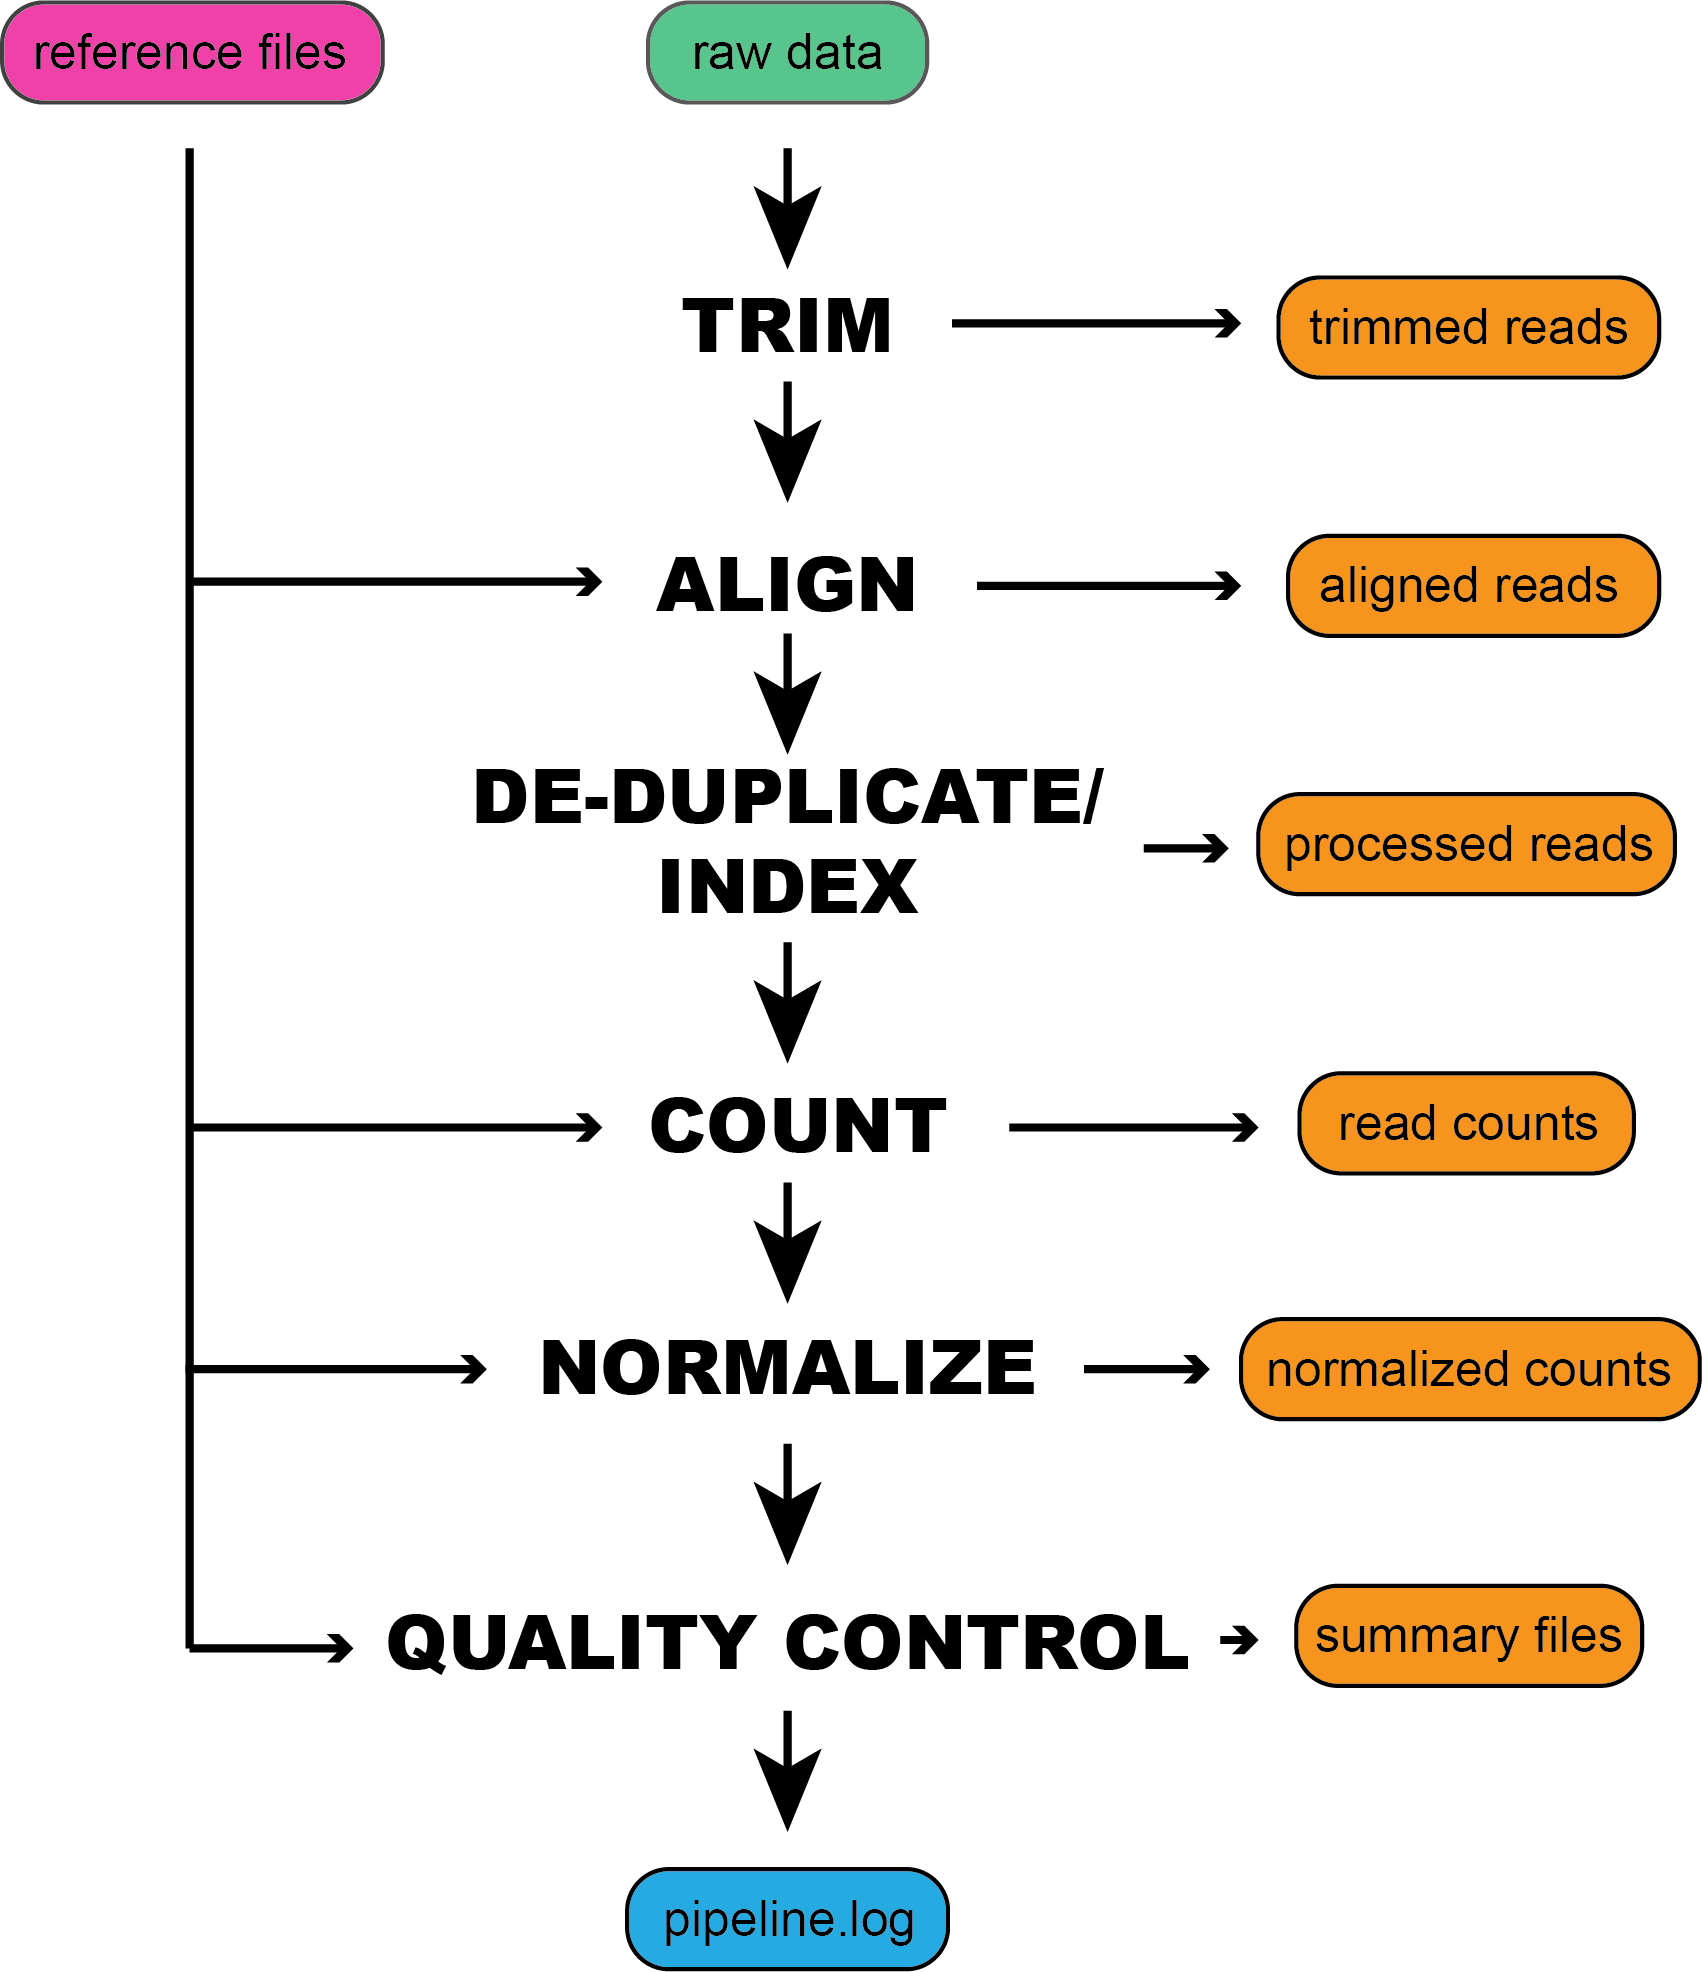
\includegraphics[width=120mm]{figures/xpresspipe_overview.png}
  \caption{An example schematic of the inputs required by XPRESSpipe and organization of the ouputs.}
  \label{fig:outputs}
\end{figure}


\subsubsection{Analyses}
XPRESSpipe has two analytical sub-modules. The first acts as a wrapper for the R package, DESeq2 \cite{deseq2}, to perform differential expression analysis on their data. More information on this sub-module can be found in the documentation (https://xpresspipe.readthedocs.io/en/latest/).

The second analytical tool introduced in XPRESSpipe is \texttt{rrnaProbe}. Ribosomal RNA (rRNA) contamination is common in RNA-seq library preparation and the bulk of RNA in a cell at any given time is dedicated to rRNA. As unique rRNA sequences are relatively few and therefore highly repeated in sequencing libraries without depletion. Depletion of these sequences is often desired in order to have better depth of coverage of mRNA sequences. In order to facilitate this depletion, many commercial kits are available that target specific rRNA sequences for depletion, or that enrich mRNA polyA tails. However, and especially in the case of ribosome profiling experiments, where RNA is digested by an RNase to create ribosome footprints, many commercial depletion kits will not perform sufficiently and polyA selection kits are inoperable as footprints will not have the requisite polyA sequence. To this end, custom rRNA probes are recommended \cite{ingolia_meth, ingolia_science}. \texttt{rrnaProbe} works on a directory containing fastqc \cite{fastqc} zip compressed files to detect over-represented sequences for each sample. These sequences are then collated to create consensus fragments. A rank ordered list of over-represented fragments within the appropriate length range to target for depletion is then output. A BLAST \cite{blast} search on consensus sequences intended for probe useage can then be performed to verify the fragment maps to an rRNA sequence and is thus a suitable depletion probe.

\subsection{XPRESSplot}
XPRESSplot is a python library of analysis features that builds upon existing packages, such as Matplotlib \cite{matplotlib} and Seaborn \cite{seaborn} to generate flexible, specific analyses and plots frequently used by biological researchers that can each be executed in a single line of code rather then tens to hundreds. Additionally, many included analytical features are currently available in an R package but not in a Python package, a programming language becoming more and more common in biological research. A summary of new or more automated tools is provided below and methods are discussed in subsequent sections. We refer the reader to the documentation (https://xpressplot.readthedocs.io/en/latest/?badge=latest) for more details instructions for other features currently in the toolkit, as well as for future features to be added.

\subsubsection{Getting Data}
XPRESSplot is designed for analyzing gene expression data, but it is tractable to most data types assuming two conditions are met:

\begin{enumerate}
  \item \textbf{Expression Matrix}: It is assumed the input data matrix = \textit{i} * \textit{j} where \textit{i} (columns) are samples and \textit{j} (rows) are genes or other relative measurement points.
  \item \textbf{Metagene Table}: It is assumed the metagene table is a two column, header-less data matrix where column 0 is the sample ID (as specified in \textit{i} of the expression matrix) and column 1 is the sample group (for example, wild-type or treatment).
\end{enumerate}

Several functions are built into XPRESSplot for importing and formatting this data. Options include importing microarray and RNA-seq expression data and metadata from the GEO database, as well as custom data and metadata that follows required formatting requirements. Several methods for normalization, such as RPM, RPKM, FPKM, TPM and log-scale normalization are accessible within this toolkit.

\subsubsection{Analyzing Data}

While a litany of analysis tools are included in XPRESSplot as of the time of writing, we will focus on tools unique to this Python library and refer to reader to the documentation for further details and examples of analysis features, current and future.

\begin{itemize}
  \item \textbf{Principle Components Analysis}: Principle components analysis (PCA) for the data matrix are performed with Python's scikit-learn package \cite{scikit_learn} and desired principle components are plotted in a scatter plot via the matplotlib \cite{matplotlib} and seaborn \cite{seaborn} packages. The XPRESSplot PCA module, as in many other analysis modules within XPRESSplot, samples are color-coded by cross-referencing the data matrix with the metagene table to determine sample label. A dictionary is additionally passed into the function that maps a particular color to each sample label. Confidence intervals are plotted over the scatterplot using numpy \cite{numpy1, numpy2} functionality as follows:

  \begin{enumerate}
    \item Compute the covariance of the two principle component arrays, \textit{x} and \textit{y} using the numpy.cov() function.

    \item Compute the eigenvalues and normalized eigenvectors of the covariance matrix using the numpy.linalg.eig() function.

    \item Compute the $\theta$ of the normalized eigenvectors using the numpy.arctan2() function and converting the output from radians to degrees using numpy.deg().

    \item Compute the $\lambda$ of the eigenvalues by taking the square root of the eigenvalues.

    \item Plot the confidence intervals over the scatter plot: The center point of the confidence interval is determined from the means of the \textit{x} and \textit{y} arrays. The angle is set equal to $\theta$. The width of the condfidence interval is calculated by
    \[
    \textit{w} = \lambda _{\textit{\scriptsize{x}}}\ \cdot\ \textit{ci}\ \cdot\ 2
    \]
    where \textit{ci} is equal to the corresponding confidence level (i.e. 68\% = 1, 95\% = 2, 99\% = 3). The heighth is similarly computed by
    \[
    \textit{h} = \lambda _{\textit{\scriptsize{y}}}\ \cdot\ \textit{ci}\ \cdot\ 2
    \]
  \end{enumerate}

  \item \textbf{Volcano Plot}: Volcano plots are an efficient method for plotting magnitude, direction, and significance of changes in expression or other data types between two conditions with multiple replicates each. By providing the categorical names for samples of two conditions in the metadata matrix, XPRESSplot will automate the calculation and plotting of this plotting method. For each gene, expression levels are averaged between the two conditions and the log\textsubscript{2}(fold change) is calculated. Additionally, for each gene, the P-value between the two conditions is calculated using scipy's individual T-test function \cite{scipy}. The log\textsubscript{2}(fold change) and -log\textsubscript{10}(P-value) is then plotted for each gene between the two conditions. Additional features available are the ability to plot threshold lines, highlight subsets of genes within the plot, and label specific genes by name.

\end{itemize}

\subsection{Availability}
The source code for these packages is open source and protected under the GPL-3.0 license. The code can be publicly accessed and installed from https://github.com/XPRESSyourself. Updates to the software are version controlled and maintained on GitHub. XPRESSplot is pip installable. XPRESSpipe is available as a Docker image. Jupyter notebooks and video walkthroughs are included on https://github.com/XPRESSyourself for guiding a user through use of the packages. Documentation is hosted on readthedocs \cite{readthedocs}.

\subsection{Cost Analysis}
Perform an example run using Docker image on AWS and give a cost per sample and time per sample output.

\subsection{Ribosome Profiling Example Data Analysis}
Only gene names in common between the original data file and XPRESSpipe output were used for the method comparisons. Genes included in all studies were required to have at least 25 counts across samples to be included in the analysis. Correlations and p-values were calculated using the \texttt{scipy.stats.spearman()} function \cite{spearman_rnaseq}. Sample count distributions were plotted using Seaborn where density is indicated by width of plot and boxplot designating interquartile range are plotted \cite{seaborn}. Fold change and translation efficiency plots were created using matplotlib \cite{matplotlib} and pandas \cite{pandas}. Replicates were combined to calculate fold change values and significance between library groups (condition and library type) was calculated using a Benjamini-Hochberg FDR method from \texttt{statsmodels.stats.multitest()} \cite{statsmodels}. Figures and analyses can be reproduced using the associated script (repo address).

\section{Results and Discussion}

\subsection{Validation}
In order to evaluate the ability of XPRESSpipe to provide the user with reliable results, we processed publicly available raw sequence files through the pipeline. We chose to highlight a ribosome profiling dataset and a subset of TCGA samples to showcase the utility of XPRESSpipe for rapidly gleaming interesting molecular patterns and insights from publicly available data.

\subsubsection{Ribosome Profiling Data and New Insights from Old Data}
The integrated stress response (ISR) is a signaling mechanism used by cells and organisms due to a variety of cellular stresses and has been associated with a variety of diseases. Of particular interest, many disorders resulting in neurological decline are associated with the ISR \cite{isr_disease}. While acute ISR is essential for proper cell survival, long periods of sustained ISR can be damaging. A recently discovered molecule, ISRIB, has recently come under the spotlight for its therapeutic potential and relative lack of side-effects. Interestingly, ISRIB is able to suppress low levels of ISR, while seemingly uneffective at managing acute, high-levels of ISR. It has also been shown to be neuroprotective in mouse models of acute neurological damage \cite{isrib_activation, isrib_structure, isrib_riboseq, isrib_neuroprotective}.

A recent study (GSE65778) utilized ribosome profiling in order to better understand the mechanisms of ISRIB and ISR, modeled by tunicamycin (Tm) treatment, from a protein translation viewpoint \cite{isrib_riboseq}. Some key findings from this study were that during acute ISR, a specific subset of mRNAs were translationally regulated, and that canonical signaling factors were part of this response. In order to showcase the utility of XPRESSpipe in analyzing ribosome profiling and sequencing datasets, we re-processed and analyzed this dataset using more current in silico techniques included in the XPRESSpipe package to shed more light on the mechanisms of ISR and ISRIB mode of action. To process the 32 raw files from GEO, using 16 cores, it took 06h33m42s in wall-clock time, or 1d03h18m27s in CPU time. Compared to the raw count data made available in the original manuscript, samples showed comparable alignment rates (Spearman R values ranging from 0.710-0.865) (Figure \ref{fig:figure2}A) as, according to the methods of the original paper, a now outdated alignment program, TopHat2 \cite{tophat2}, was used that has a documented higher false positive alignment rate compared to STAR \cite{alignment_benchmark, star}. Processing of replicates within the XPRESSpipe method showed excellent correlation (Spearman R values all \textgreater 0.99) (Figure \ref{fig:figure2}B). Additionally, samples appeared to be relatively comparable to one another once RPM normalization was performed (Figure \ref{fig:figure2}C).

\begin{figure}
\centering
  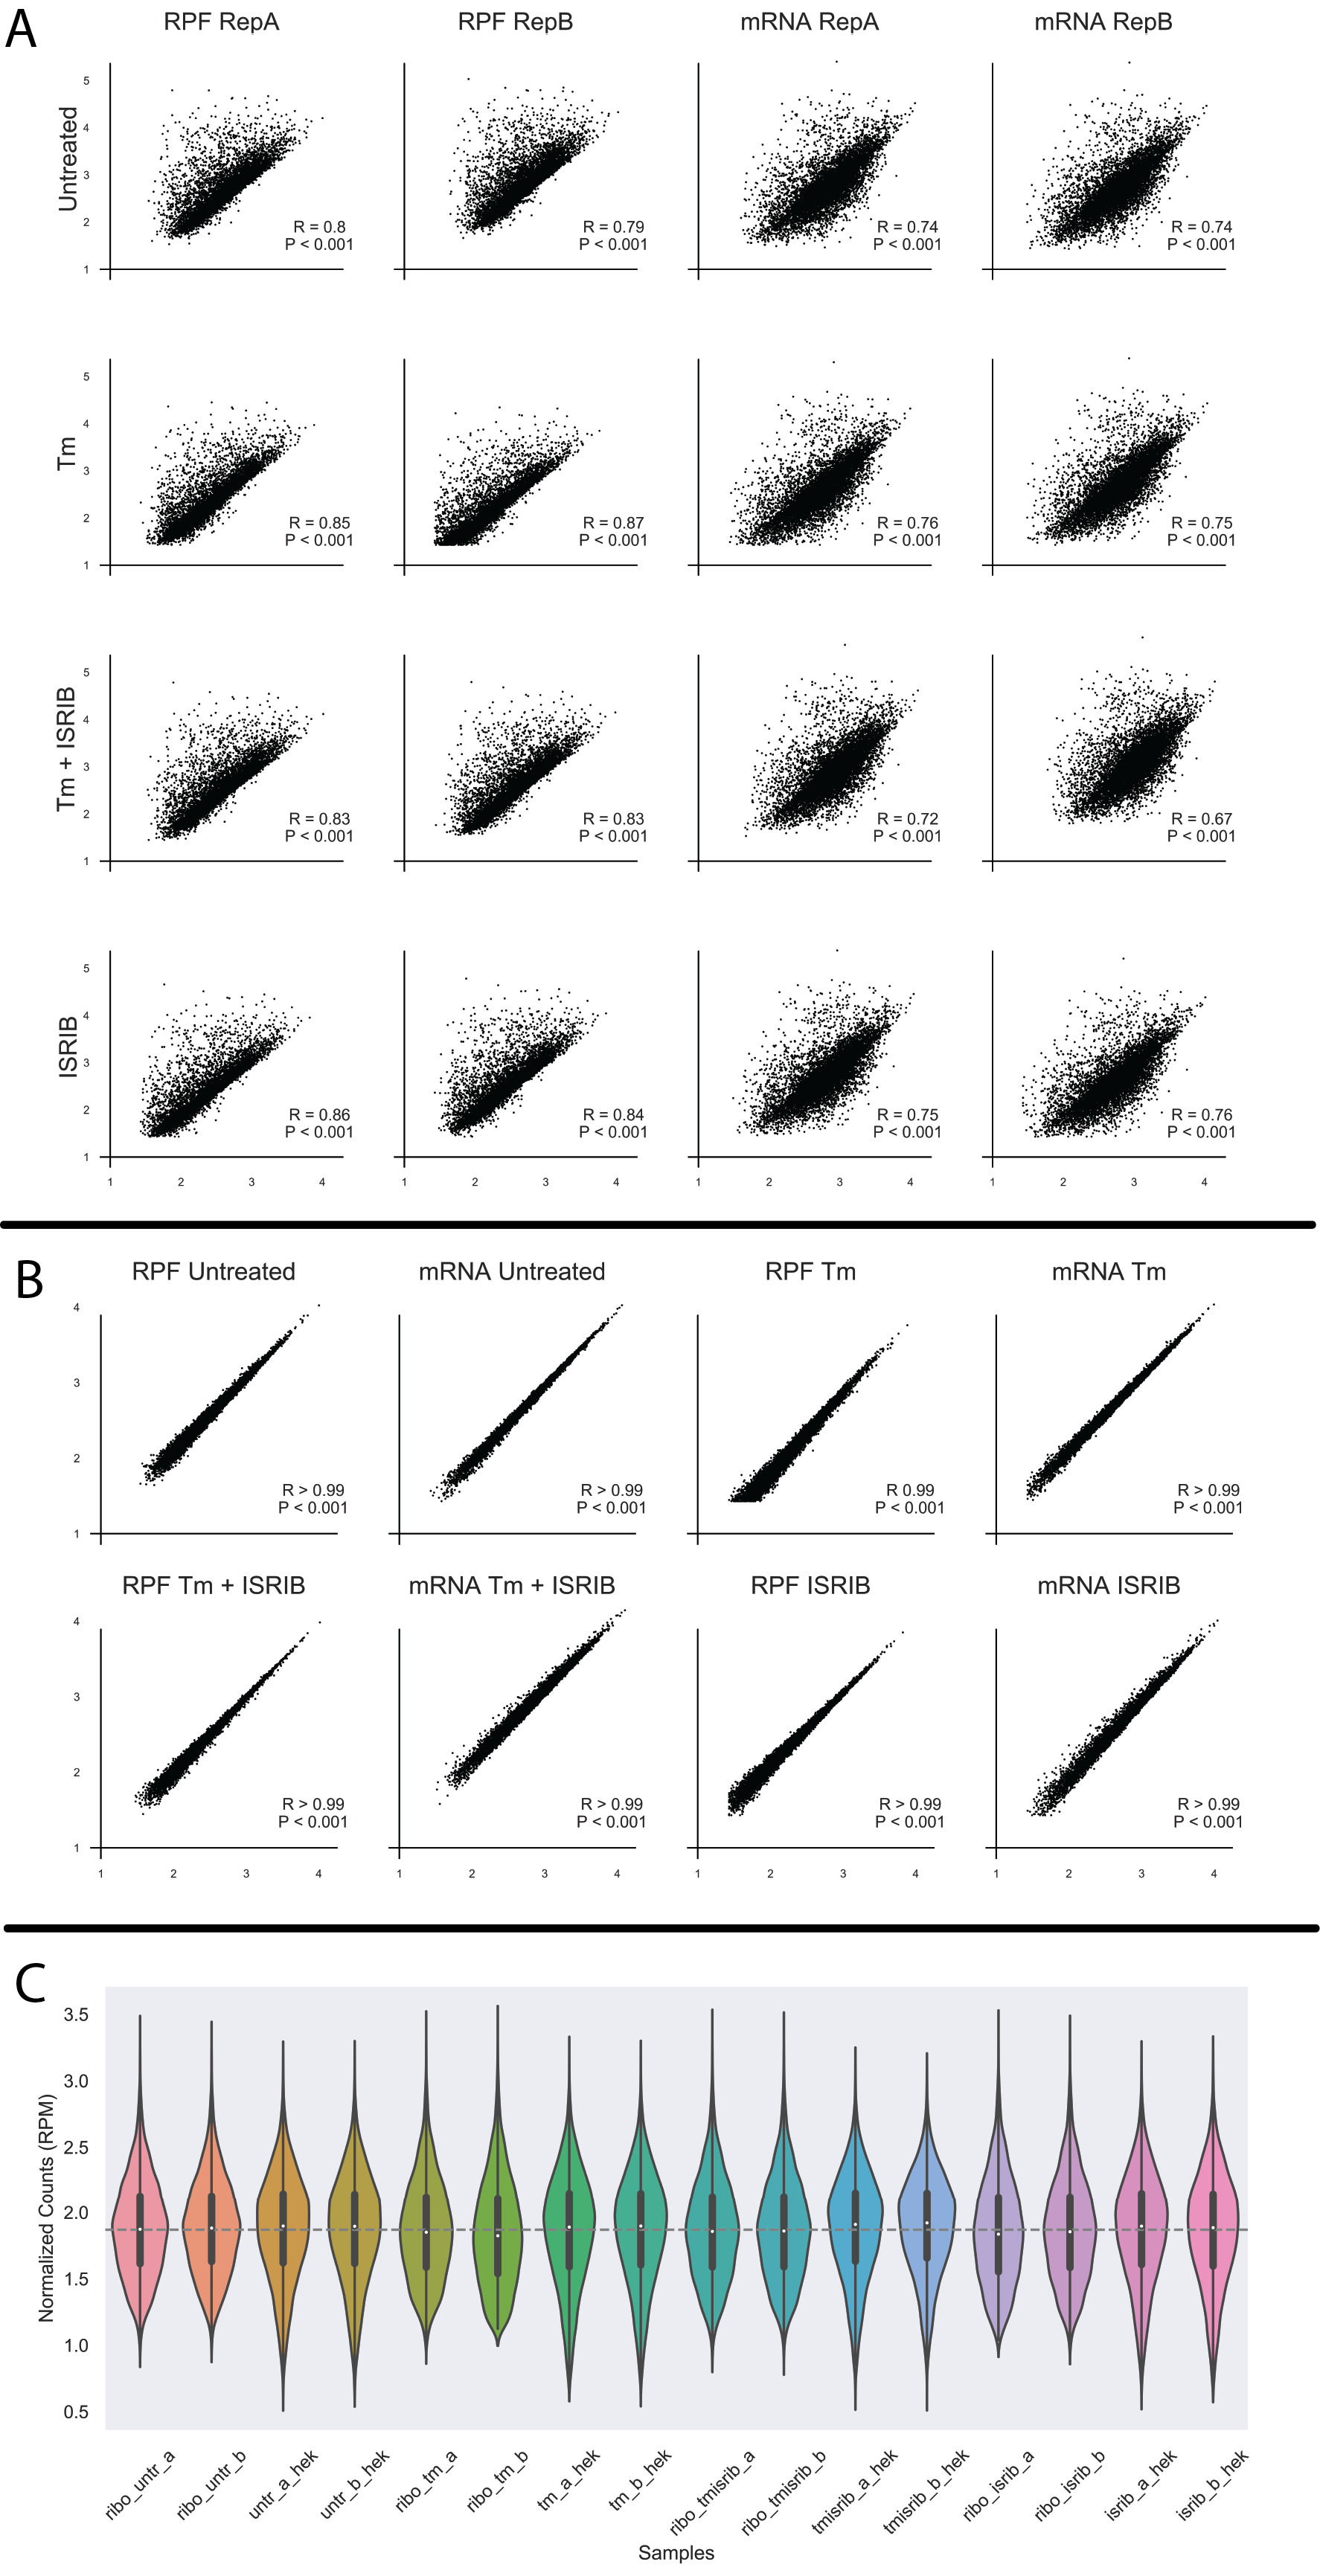
\includegraphics[width=160mm]{figures/xpresspipe_figure2.png}
  \caption{Broad sample quality control and comparision to original processing. A) Cross-processing comparisions between original manuscript and XPRESSpipe. B) Intra-processing comparisions between replicates for XPRESSpipe processing. C) Sample gene count distributions. Boxplots embedded within violinplot designate the interquartile range and violinplot reports count density. Note: All R values reported are Spearman R values.}
  \label{fig:figure2}
\end{figure}

The XPRESSpipe method interestingly showed that even more limited mRNA regulation was able to occur within the 1hr acute Tm treatment than previously appreciated (Figure \ref{fig:figure3}A), as indicated by the constrained range high-confidence (FDR \textless 0.01) points fell into along the X-axis, while the range is comparable for translation regulation. Similar canonical targets of translational regulation during ISR were identified as in the original study, such as ATF4 and ATF5 (Figure \ref{fig:figure3}A, highlighted in magenta) \cite{isrib_riboseq}. Other targets highlighted in the original study \cite{isrib_riboseq}, either narrowly missed the FDR or fold-change cut-offs or had a handful of samples with 10-25 counts for the given gene, thereby missing the stricter count cut-off, such as DDIT3 (or CHOP; fold-change = 2.09, FDR = 0.037) and PPP1R15A (or GADD34; fold-change = 1.95, FDR = 0.013). Interestingly, using these methods and thresholds, the subset of translationally down-regulated transcripts during simulated ISR all possess a neurodegenerative phenotype based on a literature search (descriptions sourced from www.genecards.org and www.omim.org) (Table \ref{tab:targets}). This might be helpful in explaining the neurodegenerative phenotype associated with ISR. When an ISR model is treated with ISRIB, the translation efficiency levels of each of these genes returns to a more wildtype-like state (Figure \ref{fig:figure3}B). Further analysis of these potential hits is strengthened by looking at the read pile-ups in IGV \cite{igv}, where footprint coverage is observed across the transcript for all ribosome profiling samples except the Tm-treated ones (Figure \ref{fig:figure3}C). This provides further strength to this claim as treatment with CircLigase in the library preparation can bias certain reads' incorporation in sequencing libraries \cite{circligase_bias}.

\begin{figure}
\centering
  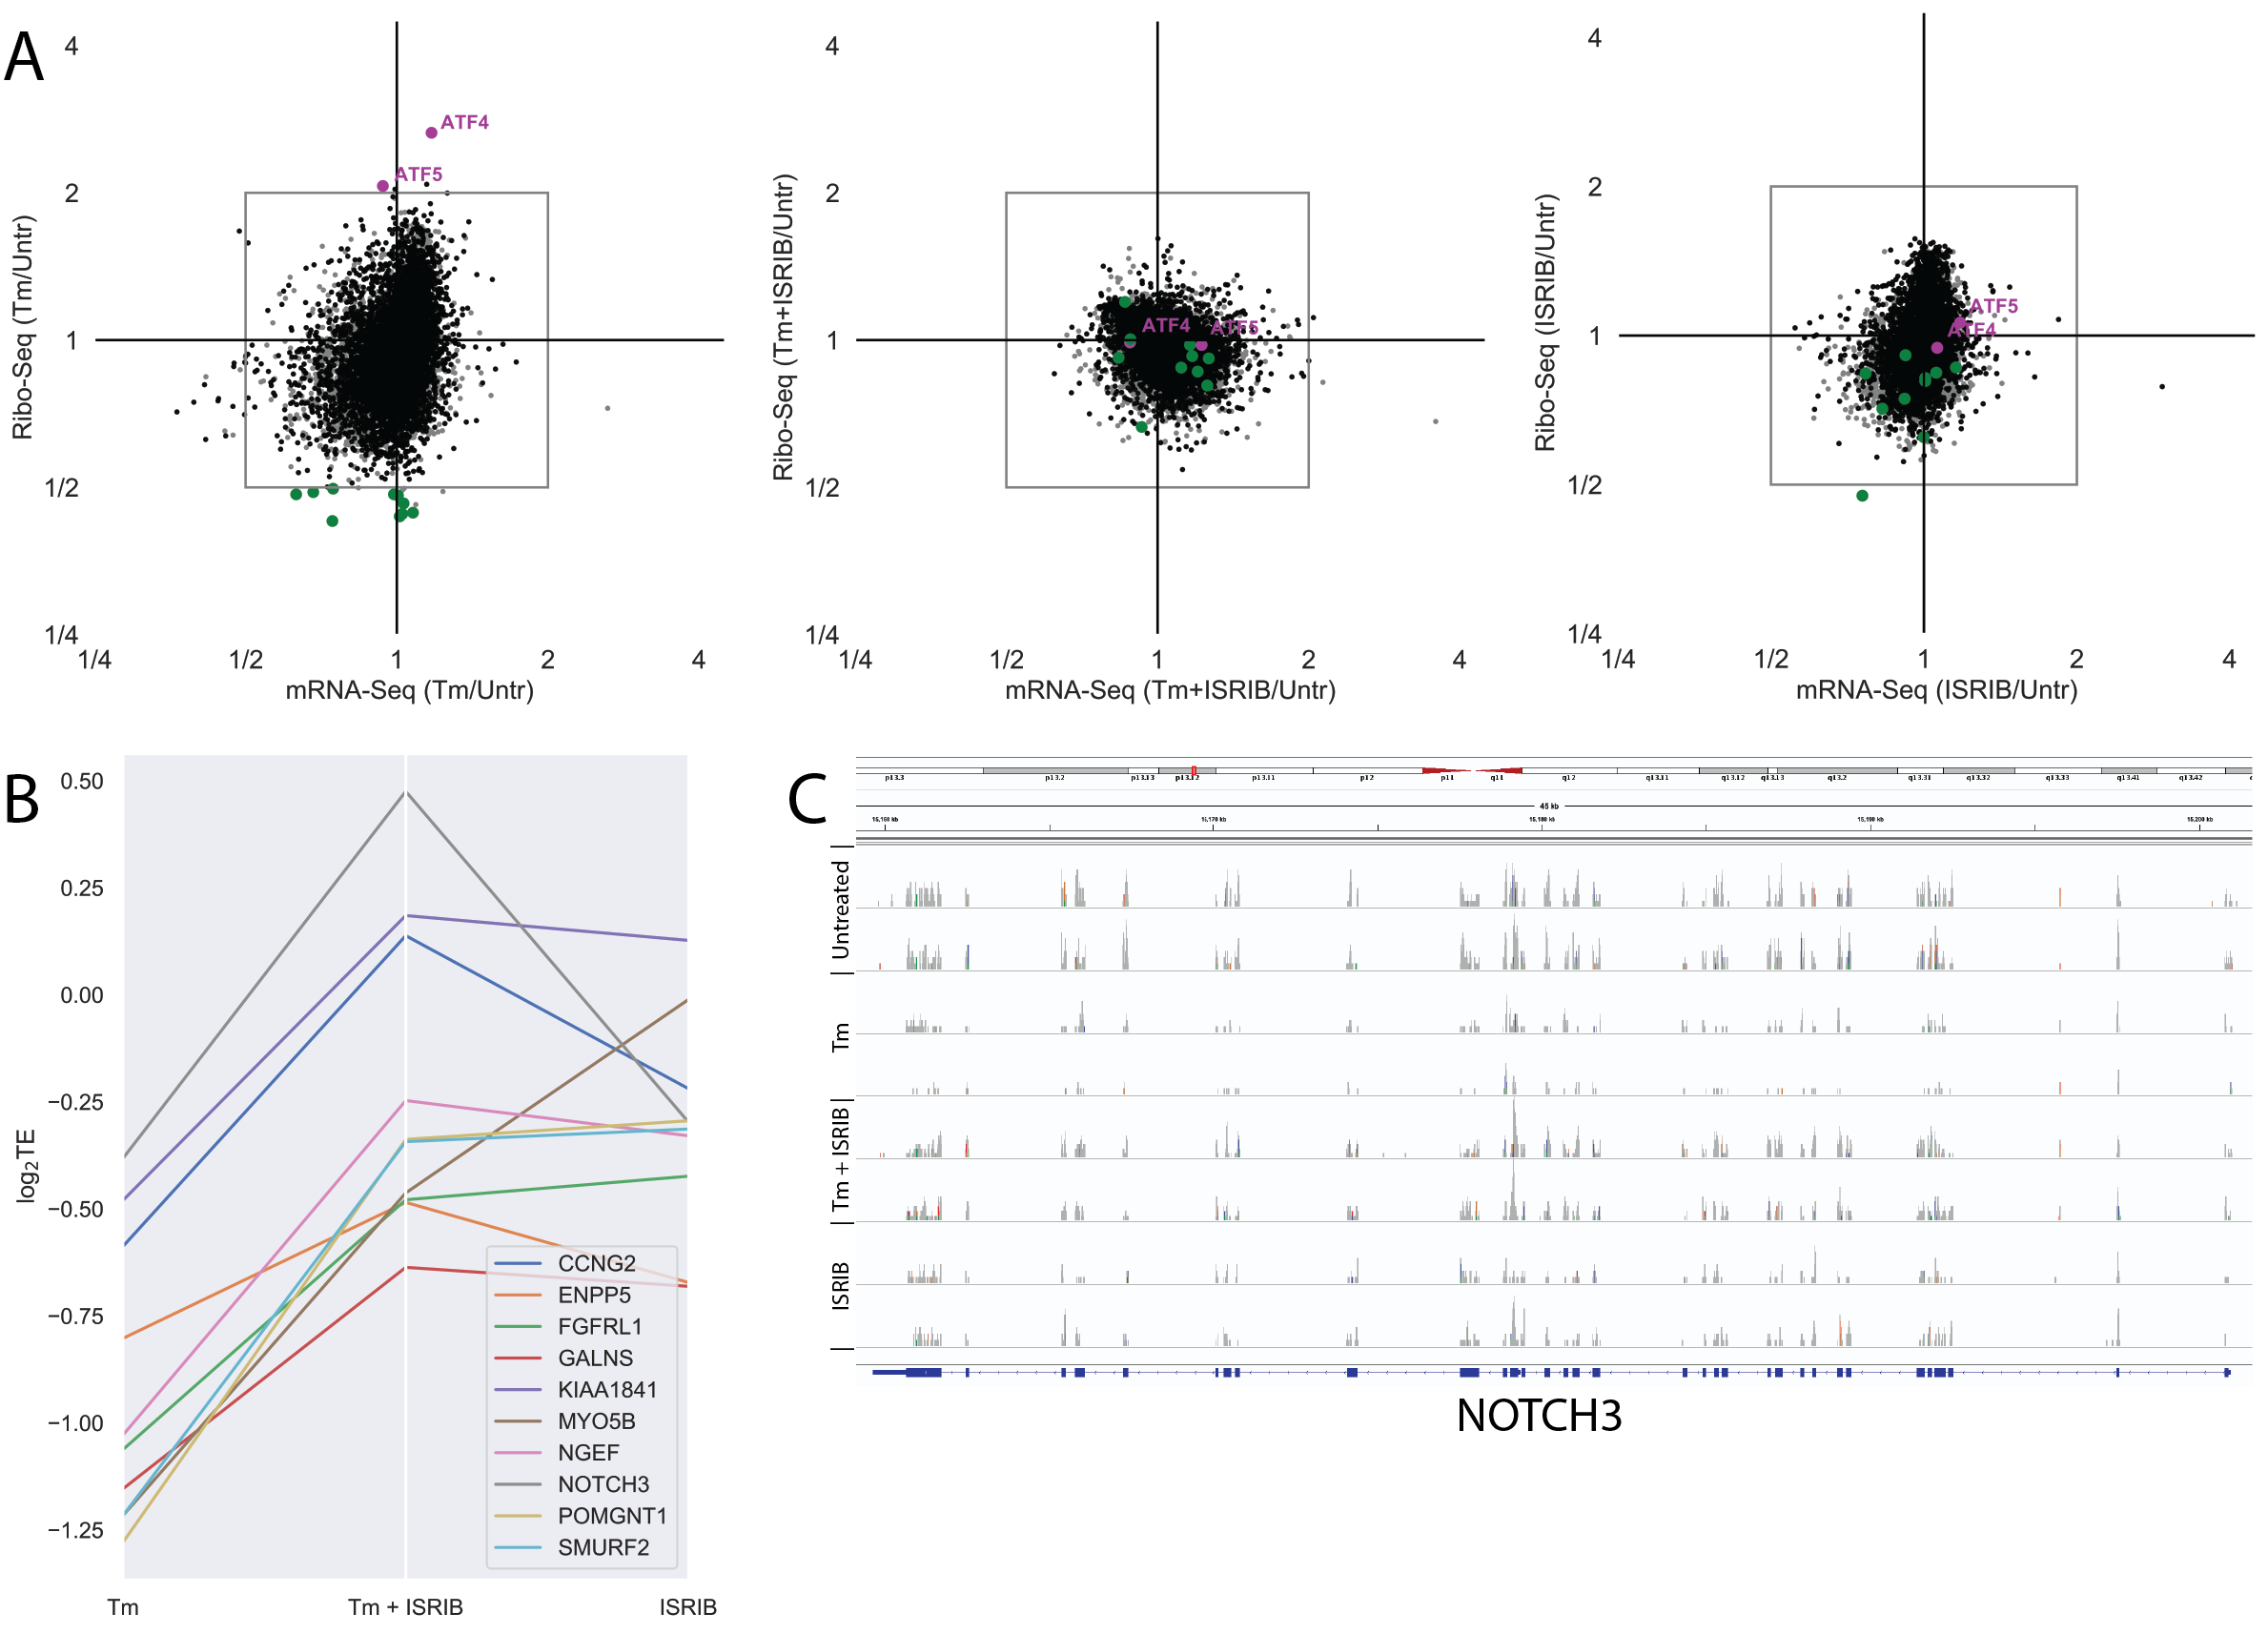
\includegraphics[width=180mm]{figures/xpresspipe_figure3.png}
  \caption{Biological validation and insight into previously published ISR model ribosome profiling data. A) Fold change for each drug condition compared to untreated for the ribosome profiling and RNA-seq data. ISR canonical targets passing fold change and significance threshold during Tm conditions are highlighted in magenta. All translationally down-regulated genes passing fold change and significance threshold during Tm conditions are highlighted in green. B) Changes in log\textsubscript{2} Translation Efficiency compared to Untreated for each drug condition for each of the translationally down-regulated genes passing previous discussed thresholds. C) IGV plot for NOTCH3 for all ribosome profiling samples show read coverage across the transcript.}
  \label{fig:figure3}
\end{figure}

\captionof{table}{Translationally down-regulated genes during acute Tm treatment.}
\begin{tabular}{p{2.5cm}p{15.5cm}}
 \textbf{Gene Name} & \textbf{Relevant Description} \\
 \hline
 CCNG2 & Overexpressed in brain; Tightly regulated in cell cycle \\
 \hline
 ENPP5 & Suggested role in neuronal cell communications in rat studies \\
 \hline
 FGFRL1 & Highly expressed in brain; Sets in motion a cascade of downstream signals ultimately influencing mitogenesis and differentiation; Behavioral and neurological phenotypes \\
 \hline
 GALNS & Involved in breaking down and recycling molecules in lysosome \\
 \hline
 KIAA1841 & Identified in a screen of proteins expressed in brain \\
 \hline
 MYO5B & Identified in a screen for large proteins expressed in brain; Encodes molecular motor that utilizes energy from ATP hydrolysis to generate mechanical force, required for the recycling of transferrin receptor back to the plasma membrane through an endocytotic recycling compartment in nonpolarized cells. \\
 \hline
 NGEF & Overexpressed in brain; Involved in axon guidance regulating ephrin-induced growth cone collapse and dendritic spine morphogenesis \\
 \hline
 NOTCH3 & Establishes an intercellular signalling pathway that plays a key role in neural development; Mutations in NOTCH3 have been identified as the underlying cause of cerebral autosomal dominant arteriopathy with subcortical infarcts and leukoencephalopathy \\
 \hline
 POMGNT1 & Mutations in this gene may be associated with muscle-eye-brain disease and several congenital muscular dystrophies \\
 \hline
 SMURF2 & Interacts with SMAD proteins; Functions in regulation of neuronal and planar cell polarity, induction of senescence, and tumor suppression \\
 \label{tab:targets}
\end{tabular}
\newline

\subsubsection{Performance Validation Using TCGA Data}
In this section, we will process the raw data for 10-20 TCGA samples and compare the FPKM counts output by XPRESSpipe to the publicly available FPKM counts for the relevant samples.
This will probably end up being added right before bioRXiv submission.

\section{Conclusions}
We have described herein a new software suite, XPRESSyourself, a collection of tools and pipelines to aid in expression data processing and analysis. We hope that with adoption of this pipeline, the field of high-throughput sequencing can arrive towards a standardized processing protocol for sequencing data and eliminate some of the variability that comes from using a variety of software packages for various steps during read processing. XPRESSpipe will act as a flexible pipeline that will be updated with the best performing packages as future tools are created and benchmarks performed. Additionally, various tools missing from the RNA-seq and ribosome profiling communities have been added as part of this pipeline. With these tools, such as the modifyGTF sub-module, genome reference curation is automated, such as creating a longest-transcript only GTF, a protein coding only GTF, or truncating the exonic ends of each transcript for use in ribosome profiling quantification. Further, by using this pipeline on publicly available data, we highlight XPRESSpipe's utility in being able to re-process publicly available data or personal data to uncover novel biological patterns quickly.

\section*{Acknowledgments}
J.A.B. received support from the National Institute of Diabetes and Digestive and Kidney Diseases (NIDDK) Inter-disciplinary Training Grant T32 Program in Computational Approaches to Diabetes and Metabolism Research, 1T32DK11096601 to Wendy W. Chapman and Simon J. Fisher. The authors wish to thank Mark Wadsworth, Ryan Miller, and Michael Cormier for helpful discussions on pipeline design. They also wish to thank Cameron Waller for helpful discussions related to pipeline design and analysis. The support and resources from the Center for High Performance Computing at the University of Utah are gratefully acknowledged.

\section*{Contributions}
\begin{tabular}{ l l }
 Conceptualization & J.A.B. \\
 \hline
 Supervision & J.P.R, M.T.H., J.G., A.R.Q. \\
 \hline
 Project Administration & J.A.B. \\
 \hline
 Investigation & J.A.B. \\
 \hline
 Formal Analysis & J.A.B. \\
 \hline
 Software & J.A.B., J.R.B. \\
 \hline
 Methodology & J.A.B., J.R.B., M.T.H., J.G. \\
 \hline
 Validation & J.A.B., J.T.M., A.J.B., Y.O. \\
 \hline
 Data Curation & J.A.B. \\
 \hline
 Resources & J.A.B. \\
 \hline
 Funding Acquisition & J.A.B. \\
 \hline
 Writing - Original Draft & J.A.B. \\
 \hline
 Writing - Review \& Editing & J.A.B., J.P.R., A.R.Q., M.T.H., J.G.,  \\
 \hline
 Visualization & J.A.B.
\end{tabular}


\bibliography{manubib}
\bibliographystyle{Science}

\end{document}
